\documentclass[10pt,fleqn]{article}
\usepackage[ruled,noline]{algorithm2e}
\usepackage[margin=1in,columnsep=20pt]{geometry}
\usepackage{amsmath}
\usepackage{amsthm}
\usepackage{amsfonts}
\usepackage{amssymb}
\usepackage{breqn}
\usepackage[
	n,
	operators,
	advantage,
	sets,
	adversary,
	landau,
	probability,
	notions,	
	logic,
	ff,
	mm,
	primitives,
	events,
	complexity,
	asymptotics,
	keys]{cryptocode}

\usetikzlibrary{trees,shapes,decorations,graphs,matrix}

\usepackage{float}
%\usepackage{url}
\usepackage{hyperref}

\title{Extended Abstract: An Anonymous Payment Scheme with BFTKV}
\author{%
  \textsc{Ryuji Ishiguro}\\%
}
\date{{\small -- Very Preliminary (ver 0.3) --}}

\begin{document}
\maketitle

\begin{abstract}

This is an extension of \textsf{bftkv} \cite{bftkv}. We show that our Byzantine fault-tolerant key-value store can be an efficient and scalable solution for Bitcon like trasactions. On top of that, we develop an anonymous payment scheme. In our scheme, anonymity and confidentiality are built-in, not an add-on. We use a ZKP technique not only to make the transaction confidential but also to ensure the validity of transactions, which is usually done using digital signatures. There is not any linkable information in the transaction such as ``addresses'' to be hidden in the first place. The double spending problem is reduced to the equivocation problem that is solved with \textsf{bftkv}.

\end{abstract}

\section{Introduction}
All transactions are stored in the global ledger in the PoW type blockchains to make PoW efficient. Even if the addresses are pseudonym it is easy to track the transactions. Also each transaction includes the amount of coins that are transferred from an address to another address so even 3rd party entities can know exactly how much coin is spent or kept by an address. This is the way to check that someone is not cheating in blockchains like Bitcoin. Even non PoW type blockchains, most of which are based on BFT state machine replication (such as PBFT \cite{pbft}), follow the same mechanism when it comes to transactions. We take an advantage of Byzantine fault-tolerant KV store. First of all, your transaction is known by only you and someone you are trading with, and it does not have to be published to all over the world. Payers and payees verify a transaction themselves and stores it in the KV store with a ``Proof of Balance''. The KV slots are ``write once'' so any other transactions cannot overwrite it. This feature of \textsf{bftkv} can be equivalent to the global ledger but unlike PoW or state machine replication it does not require absolute constency among participants. This makes it easy to scale the system. 

As above, we introduce a new consensus mechanism called Proof of Balance or PoB to add transactions to the global ledger (which is, in our case, the KV store). Once a pair of key (balance) - value (transaction) is verified (with PoB), accepted (with the quorum) and stored in the leger (KV store), we consider the system reaches a consensus on the validity of the transaction with the balance. We use a Zero Knowledge Proof technique to construct PoB. This scheme does not require any long term key such as signing keys and the transaction does not include any linkable information such as signatures or public keys. We discuss anonymity later. The balance is encrypted and never decrypted in any way. All we have to consider is the total balance before and after a transaction. We do not have to know the actual balance of others. ZKP makes it possible to calculate the balance on encrypted data. 

We do not have a hash chain. Instead, the KV relation forms a DAG where the vertices are encrypted balances and the edges are transactions, which we call Chain of Balance. PoW bonds the balances so without PoW no vertix can be inserted. We can verify the soundness of the payment system by tracing the graph. (See \nameref{Audit}.)

\section{Recap of \textsf{bftkv}}
A quick reqcap of the building blocks of \textsf{bftkv}.

\subsubsection*{Quorum Cliques}

\textsf{bftkv} follows the idea of byzantine quorum \cite{byzantinequorum}. Our quorum system is constructed by the trust graph (Web of Trust) and ``Quorum Clique'' is the fundamental building block. The quorum clique is a sub-graph, that is $G_C = (V, E)$, where
\begin{enumerate}
\item For $\forall v_i, v_j \in V, (v_i, v_j) \text{ and } (v_j, v_i) \in E$,
\item $|V| \ge 4$,
\item $\forall v \in V$ is not a member of any other quorum clique.
\end{enumerate}
With these conditions, an attempt of sybil attacks ends up splitting a clique.

\begin{figure}[h]
\begin{center}
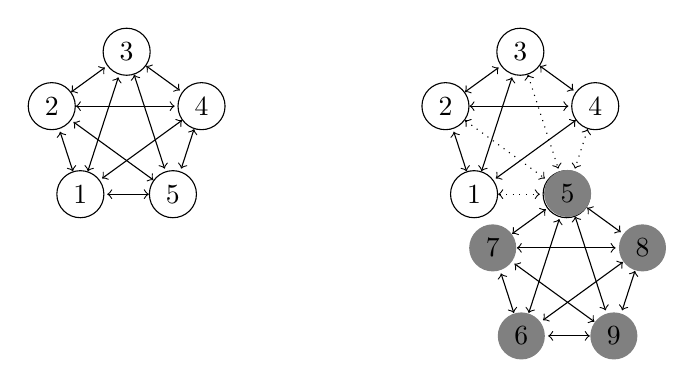
\begin{tikzpicture}[shorten >=1pt,<->]
  \tikzstyle{vertex}=[circle,minimum size=17pt,inner sep=0pt]

  \foreach \name/\angle/\text in {R-1/234/1, R-2/162/2, R-3/90/3, R-4/18/4, R-5/-54/5}
    \node[vertex,xshift=6cm,yshift=.5cm,draw] (\name) at (\angle:1cm) {$\text$};

  \foreach \name/\angle/\text in {P-1/234/1, P-2/162/2, P-3/90/3, P-4/18/4, P-5/-54/{}}
    \node[vertex,xshift=11cm,yshift=.5cm,draw] (\name) at (\angle:1cm) {$\text$};

  \foreach \name/\angle/\text in {Q-1/234/6, Q-2/162/7, Q-3/90/5, Q-4/18/8, Q-5/-54/9}
    \node[vertex,xshift=11.6cm,yshift=-1.3cm,fill=gray] (\name) at (\angle:1cm) {$\text$};

  \foreach \from/\to in {1/2,2/3,3/4,4/5,5/1,1/3,2/4,3/5,4/1,5/2}
    { \draw (R-\from) -- (R-\to); }

  \foreach \from/\to in {1/2,2/3,3/4,1/3,2/4,4/1}
    { \draw (P-\from) --  (P-\to); }

  \foreach \from/\to in {1/5,2/5/,3/5,4/5}
    { \draw [dotted] (P-\from) ->  (P-\to); }

  \foreach \from/\to in {1/2,2/3,3/4,4/5,5/1,1/3,2/4,3/5,4/1,5/2}
    { \draw (Q-\from) -- (Q-\to); }
\end{tikzpicture}
\end{center}
\caption{Quorum Clique}
\end{figure}
The left clique is a legitimate one. When the node 5 is compromised and the attacker attempts to outnumber the legitimate nodes with colluding nodes (node 6..9). Since the node 5 cannot be a memeber of another clique the attacker has no choice but severing the trust links. The end result is we have two separated cliques and it does not affect the legitimate cliques.

\subsubsection*{Quorum Certificates}
Quorum certificates are collective certificates signed by the members of quorum cliques. When a node joins the network a quorum certificate is issued and it represents a trust graph rooted by the node.

\subsubsection*{Key-value Quorum}
Once a triple $\langle x, t, v \rangle$ is signed by a quorum clique, it will be stored in other nodes ($\notin QC$). These nodes form another quorum system, called ``KV quorum''. In our system this quorum system plays a role of the auditor as well. Each node checks equivocation before storing the triple and if it finds a malicious action it revokes the member and propagates a proof of malicious actions. Once a member is revoked there is no way to re-join the network.

\subsubsection*{Revocation}
Each legitmate node must check equivication. Malicious nodes could sign a different value for the same variable and timestamp, i.e., $\langle x, t, v \rangle$ and $\langle x, t, v' \rangle$ where $v \ne v'$. Such equivocation can be detected when it's stored in KV quorum. Another type of equivocation is to show other nodes a different view of the trust graph. To detect such attack, each node should keep its own view of the trust graph and whenever it receives the quorum certificate it checks if it's consitent with its own graph and udpates it if it finds an updated nodes in the QC.

\subsection{Read / Write Protocols}
The transport security is out of scope of this proposal. Without any additional security scheme the protocol has to be secure by itself. But in a real world situation we need to consider additional security measures. Imagine that you are connecting a public WiFi at a cafe and this network is totally controled by a malicious attacker. Even if the attacker cannot forge the message they can do some common attacks such as reply attack and relay attack. If we only rely on the quorum system this situation looks like a case where all nodes are faulty. To mitigate this kind of situation we add a simple challenge-response protocol with a nonce.

In addition to the transport level security, we add a simple gossip among nodes in the KV quorum. Gossip is voluntary and the system does not rely on how gossip propagate the message, but this is a good way to keep the whole network sound and secure. We use gossip to extend the \textsf{write} protocol and propagate the revocation message.

\subsubsection*{Write}
The write operation is done among the client, Quorum Clique and KV quorum. 

\begin{figure}[H]
\begin{center}
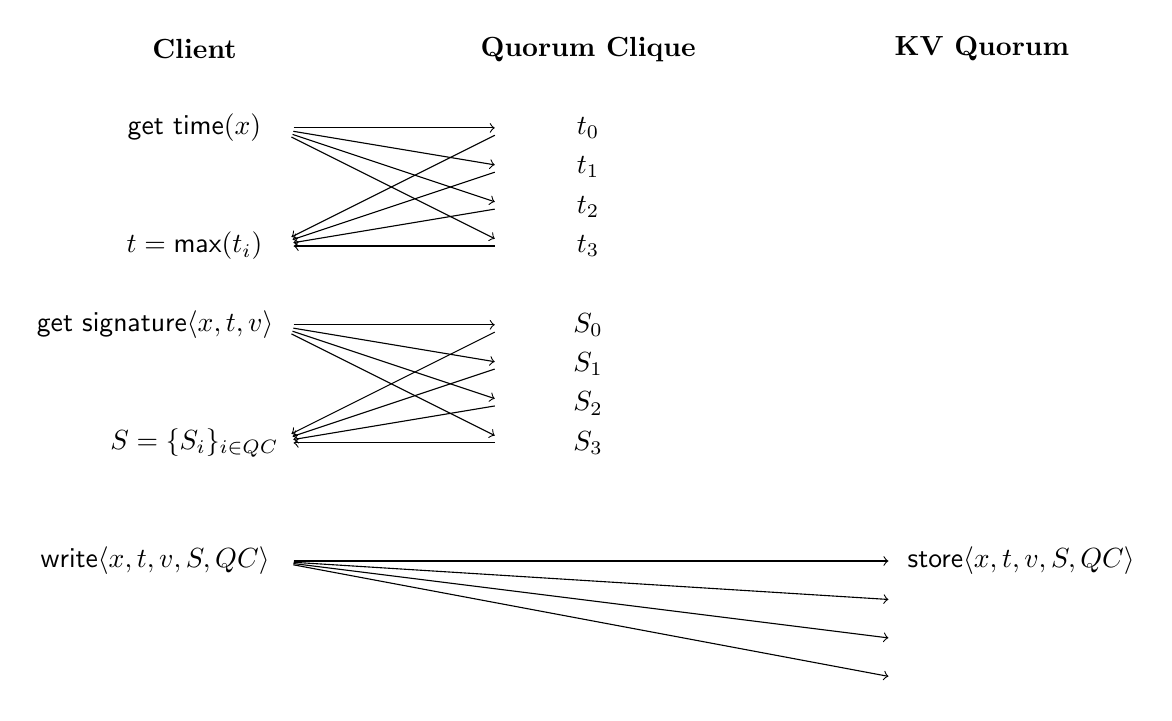
\begin{tikzpicture}
  \draw (-1,1) node {\textbf{Client}};
  \draw (4,1)  node {\textbf{Quorum Clique}};
  \draw (9,1)  node {\textbf{KV Quorum}};

  \draw (-1,0) node {\textsf{get time}$(x)$};
  \draw (-1,-1.5) node {$t = \textsf{max}(t_i)$};

  \node[shape=circle,scale=1.5] (A) at (0,0) {};
  \node[shape=circle,scale=1.5] (B) at (0,-1.5) {};
  \foreach \to/\i in {0/0, -0.5/1, -1/2, -1.5/3} {
    \node[scale=1.5] (C) at (3,\to) {};
    \draw[->] (A) -- (C);
    \draw[->] (C) -- (B);
    \draw (4,\to) node {\textsf{$t_\i$}};
  }

  \draw (-1.5,-2.5) node {\textsf{get signature}$\langle x, t, v \rangle$};
  \draw (-1,-4) node {$S = \{S_i\}_{i \in QC}$};

  \node[shape=circle,scale=1.5] (A) at (0,-2.5) {};
  \node[shape=circle,scale=1.5] (B) at (0,-4) {};
  \foreach \to/\i in {-2.5/0, -3/1, -3.5/2, -4/3} {
    \node[scale=1.5] (C) at (3,\to) {};
    \draw[->] (A) -- (C);
    \draw[->] (C) -- (B);
    \draw (4,\to) node {\textsf{$S_\i$}};
  }

  \draw (-1.5,-5.5) node {\textsf{write}$\langle x, t, v, S, QC \rangle$};

  \node[shape=circle,scale=1.5] (A) at (0,-5.5) {};
  \foreach \to in {-5.5,-6,-6.5,-7} {
    \node[scale=1.5] (C) at (8,\to) {};
    \draw[->] (A) -- (C);
  }

  \draw (9.5,-5.5) node {\textsf{store}$\langle x, t, v, S, QC \rangle$};

\end{tikzpicture}
\end{center}
\caption{Write Protocol}
\end{figure}

Each member of KV quorum does the equivocation check. If the check fails it will propagate a revocation message instead of the signed triple to other members. 
The system does not provide absolute or eventual consistency unlike state machine replication. The communication complexity is $\bigO{N}$ or $\bigsmallO{|Q|}$ at the time of read / write. The system asynchronously gossips the signed triple and revocation state. The client does not wait for the reply from the quorum members to conclude a transaction. See the risk analysis. This way we can scale the system without increasing communication complexity beyond the limitation of the quorum threadhold.

Each member of Quorum Clique checks if $\langle x, t \rangle$ has been already used to sign. If a client makes such a request that is attempting to make a equivocation the client will be revoked, though this kind of malicious action is too obvious.  Typical ``malicious'' actions will be found by KV quorum (5. Security Analysis \cite{bftkv}). 

\subsubsection*{Read}
The read operation is done between the client and KV quorum.

\begin{figure}[H]
\begin{center}
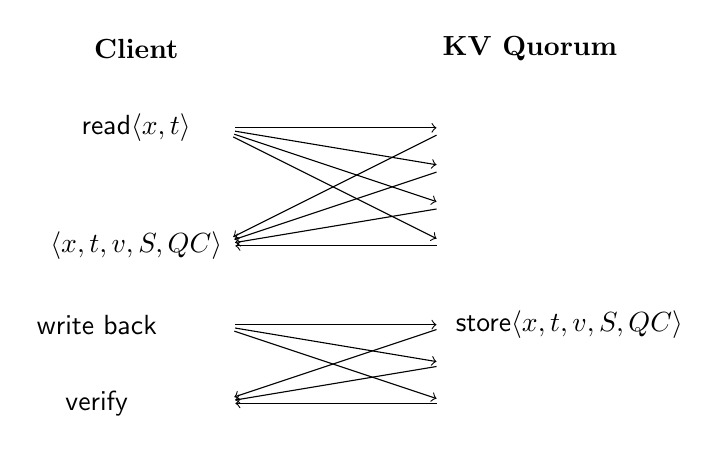
\begin{tikzpicture}
  \draw (-1,1) node {\textbf{Client}};
  \draw (4,1)  node {\textbf{KV Quorum}};
  
  \draw (-1,0) node {\textsf{read}$\langle x, t \rangle$};
  \draw (-1,-1.5) node {$\langle x, t, v, S, QC \rangle$};

  \node[shape=circle,scale=1.5] (A) at (0,0) {};
  \node[shape=circle,scale=1.5] (B) at (0,-1.5) {};
  \foreach \to/\i in {0/0, -0.5/1, -1/2, -1.5/3} {
    \node[scale=1.5] (C) at (3,\to) {};
    \draw[->] (A) -- (C);
    \draw[->] (C) -- (B);
  }

  \draw (-1.5,-2.5) node {\textsf{write back}};
  \draw (4.5,-2.5) node {\textsf{store}$\langle x, t, v, S, QC \rangle$};

  \node[shape=circle,scale=1.5] (A) at (0,-2.5) {};
  \node[shape=circle,scale=1.5] (B) at (0,-3.5) {};
  \foreach \to/\i in {-2.5/0, -3/1, -3.5/2} {
    \node[scale=1.5] (C) at (3,\to) {};
    \draw[->] (A) -- (C);
    \draw[->] (C) -- (B);
  }

  \draw (-1.5,-3.5) node {\textsf{verify}};

\end{tikzpicture}
\end{center}
\caption{Read Protocol}
\end{figure}

\section{Payment Scheme}
As stated in Introduction our payment scheme is strictly peer-to-peer and only the result of transactions, which is a new balance, is written in the KV quorum. The image of a trasaction may look like this:
\begin{figure}[H]
\begin{center}
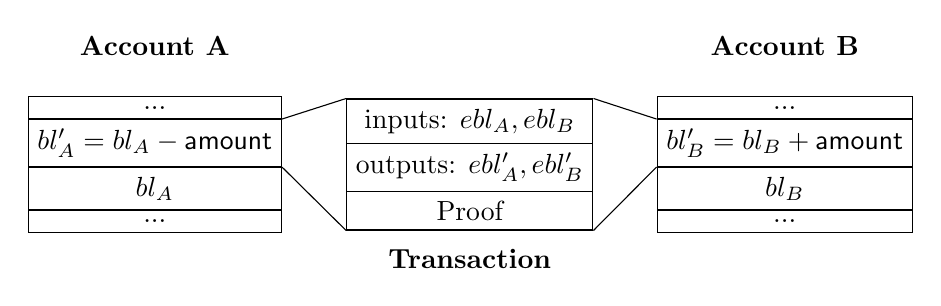
\begin{tikzpicture}[stack/.style={rectangle split, rectangle split parts=#1,draw, anchor=center}]

  \draw (0,1.5) node {\textbf{Account A}};
  \node[stack=4] (A) at (0,0) {
    \nodepart{one}...
    \nodepart{two} $bl_A' = bl_A - \textsf{amount}$
    \nodepart{three} $bl_A$
    \nodepart{four} ...
  };

  \node[stack=3, 
        every one node part/.style={fill=gray}] (B) at (4, 0) {
    \nodepart{one} {inputs: $ebl_A, ebl_B$}
    \nodepart{two} {outputs: $ebl_A', ebl_B'$}
    \nodepart{three} {Proof}
  };
  \draw (4,-1.2) node {\textbf{Transaction}};

  \draw (8,1.5) node {\textbf{Account B}};
  \node[stack=4] (C) at (8,0) {
    \nodepart{one}...
    \nodepart{two} $bl_B' = bl_B + \textsf{amount}$
    \nodepart{three} $bl_B$
    \nodepart{four} ...
  };

  \draw[-] (A.one split east) -- (B.north west);
  \draw[-] (A.two split east) -- (B.south west);
  \draw[-] (B.north east) -- (C.one split west);
  \draw[-] (B.south east) -- (C.two split west);

\end{tikzpicture}
\end{center}
\caption{Balance based Transaction}
\end{figure}

\textbf{A} pays \textsf{amount} to \textbf{B} ``out of band'' or in a peer-to-peer manner. This payment protocol is discussed later in this section. \textsf{Proof} is a Zero Knowlege Proof of the existance of $bl$ and $bl'$. We discuss the ZK Proof of the balance in detail below. The total balance is calculated over $ebl$ which is an encryption of $bl$, without decrypting it. By verifying the proof we know the total balance has not changed before and after the transaction and any balance is not negative, i.e.,
\[
(\sum{\textsf{bl}_i} = \sum{\textsf{bl}_i'} ) \wedge (\textsf{bl}_i' \ge 0).
\]

The quorum system is used to prevent double spending. Specifically we use the ``write once'' feature of \textsf{bftkv}. We also add an anonymous write feature to write once. Since the variable is never modified it can be written without the owner's quorum certificate.

\subsection{Zero Knowledge Proof of Balance (zkPoB)}
As above, each entity does not have to know the balance of other parties. They only need to know that the total balance has not changed before and after a transaction.  We use a ZKP technique to calculate the total balance without letting others know the actual value. Also we need to make sure that each balance is in a certain range so that a negative balance is detected. Putting them together the relation can be:

\[
\begin{split}
\mathcal{R} := \{& ((bl_i, bl_i', \beta_i, \beta_i'), (u, e_i, e_i')) : \\
& e_i = u^{\beta_i}g^{bl_i}, e_i' = u^{\beta_i'}g^{bl_i'}, 0 \le bl_i' < 2^d, \text{ and } \sum_i bl_i = \sum_i bl_i' \}.
\end{split}
\]
With this relation, we have:
\[
\begin{split}
(u, e_i, e_i') \in L_{\mathcal{R}} \Longleftrightarrow & \; \prod_i e_i / \prod_i e_i' = \prod_i u^{\beta_i} u^{-\beta_i'} = \prod_i u^{\beta_{\triangle
      i}}, \\ & \text{where } \beta_{\triangle i} = \beta_i - \beta_i',
\end{split}
\]
if and only if $\sum_i bl_i = \sum_i bl_i'$. Therefore all we need to
do is to run a sigma protocol to prove that each party has
$\beta_{\triangle i}$, i.e.,
\[
\mathcal{R}' := \{ ((\beta_{\triangle i}, bl_i', \gamma_i), (u, w_i, b_{ij}, c_{ij})) : w_i = u^{\beta_{\triangle i}}, c_{ij} = u^{\gamma_i} g^{b_{ij}} \}
\]
that satisfies:
\[
(\prod_i e_i / \prod_i e_i' = \prod_i w_i) \wedge (bl_i' = \sum_{j = 0..d-1} 2^{j} b_{ij}).
\]
The Sigma protocol of PoB will look like the Figure \ref{PoB}.

\begin{figure}[h]
\begin{center}
  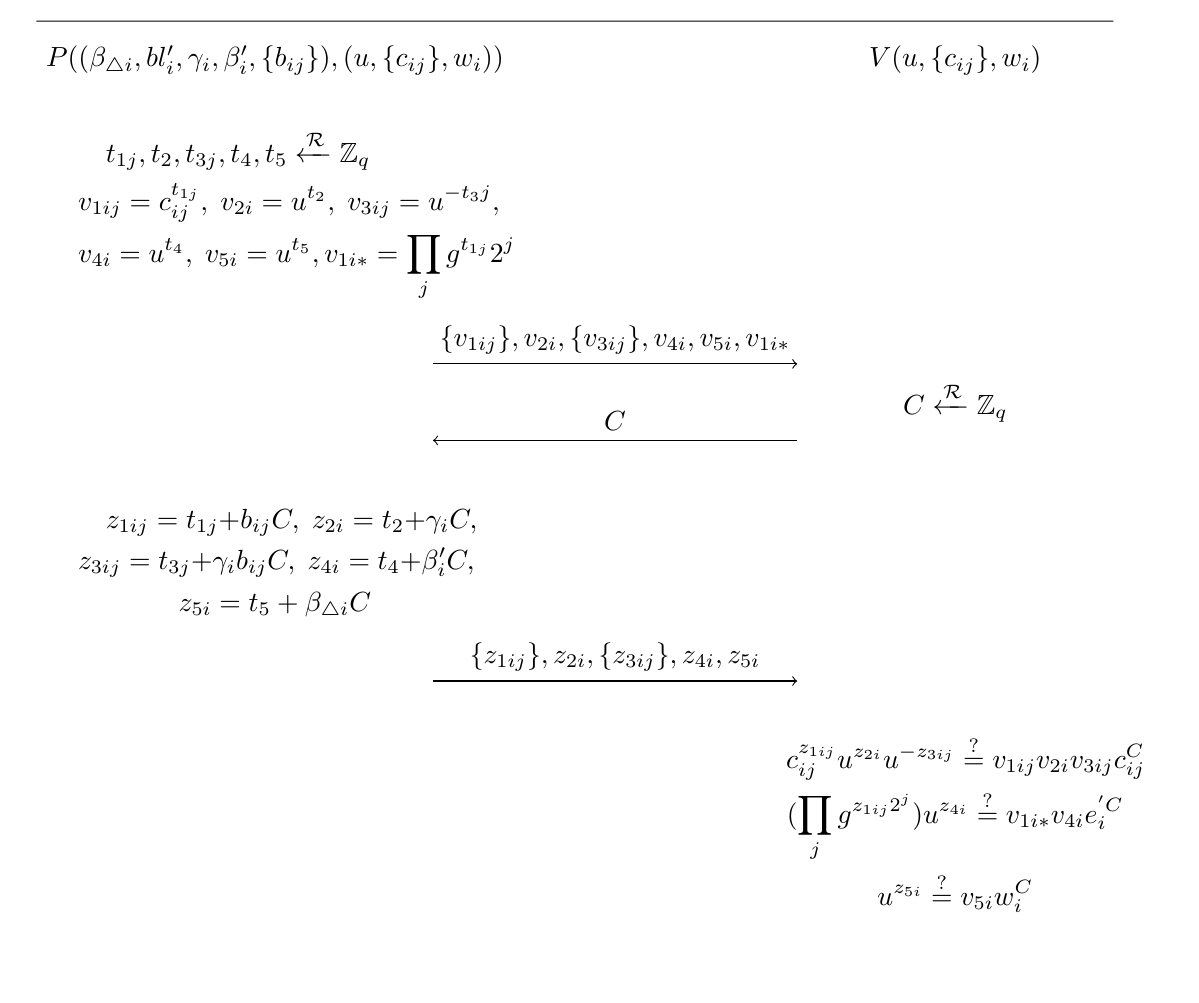
\begin{tikzpicture}
    \matrix (m) [matrix of math nodes, nodes in empty cells, row
      sep=0cm, column sep=3cm, minimum width=4cm] {
      P((\beta_{\triangle i}, bl_i', \gamma_i, \beta_i', \{b_{ij}\}), (u, \{c_{ij}\}, w_i)) & V(u, \{c_{ij}\}, w_i) \\
      \begin{minipage} {5cm} \begin{multline*}
          t_{1j}, t_2, t_{3j}, t_4, t_5 \xleftarrow{\mathcal{R}} \mathbb{Z}_q \\
          v_{1ij} = c_{ij}^{t_{1j}}, \; v_{2i} = u^{t_2}, \; v_{3ij} = u^{-t_3j}, \\
          v_{4i} = u^{t_4}, \; v_{5i} = u^{t_5}, v_{1i*} = \prod_j g^{t_{1j}} 2^j \\
      \end{multline*} \end{minipage}  & \\
                      & \\
                      & C \xleftarrow{\mathcal{R}} \mathbb{Z}_q \\
                      & \\
      \begin{minipage} {5cm} \begin{multline*}
          z_{1ij} = t_{1j} + b_{ij} C, \; z_{2i} = t_2 + \gamma_i C, \\
          z_{3ij} = t_{3j} + \gamma_i b_{ij} C, \; z_{4i} = t_4 + \beta_i' C, \\
          z_{5i} = t_5 + \beta_{\triangle i} C \\
      \end{multline*} \end{minipage}  & \\
                      & \\
                      & \begin{minipage}{5cm} \begin{multline*}
                            c_{ij}^{z_{1ij}} u^{z_{2i}} u^{-z_{3ij}} \overset{?}{=} v_{1ij} v_{2i} v_{3ij} c_{ij}^C \\
                            (\prod_j g^{z_{1ij} 2^j}) u^{z_{4i}} \overset{?}{=} v_{1i*} v_{4i} e_i^{'C} \\
                            u^{z_{5i}} \overset{?}{=} v_{5i} w_i^C \\
                        \end{multline*} \end{minipage} \\
    };

    \draw [-, transform canvas={yshift=0.5cm}] (m-1-1.west) -- (m-1-2.east) node [very near start, above] {};
    \draw [->] (m-3-1) -- (m-3-2) node [midway, above] {$\{v_{1ij}\}, v_{2i}, \{v_{3ij}\}, v_{4i}, v_{5i}, v_{1i*}$};
    \draw [<-] (m-5-1) -- (m-5-2) node [midway, above] {$C$};
    \draw [->] (m-7-1) -- (m-7-2) node [midway, above] {$\{z_{1ij}\}, z_{2i}, \{z_{3ij}\}, z_{4i}, z_{5i}$};
  \end{tikzpicture}
\caption{Sigma Protocol for PoB}
\label{PoB}
\end{center}
\end{figure}
After finishing the protocol with all parties, check if $\prod_i e_i / \prod_i e_i' \overset{?}{=} \prod_i w_i$.

\subsection{Payment Protocols}
We define the transaction as follows:
\begin{multline*}
PoB_i := ((u, \{c_{ij}\}_j, w_i), (\{v_{1ij}\}_j, v_{2i}, \{v_{3ij}\}_j, v_{4i}, v_{5i}, \{z_{1ij}\}_j, z_{2i}, \{z_{3ij}\}_j, z_{4i}, z_{5i})) \; (j = 0..d-1) \\
Tx := \{ebl_i, ebl_i', PoB_i \}_i \\
\end{multline*}
$ebl_i, ebl_i'$ for some $i$ can be \textsf{nil} which is treated as $bl=0$. We use the Fiat-Shamir transform to convert the Sigma Protocol \ref{PoB} to $PoB$.

The Figure \ref{payment_example} is a payment example: A and B jointly pay \$2 and \$3 to C. This transaction creates a brand new balance for C. Whatever $bl_A$ and $bl_B$ are, the total balance of A, B, and C does not change.
\begin{figure}[H]
\begin{center}
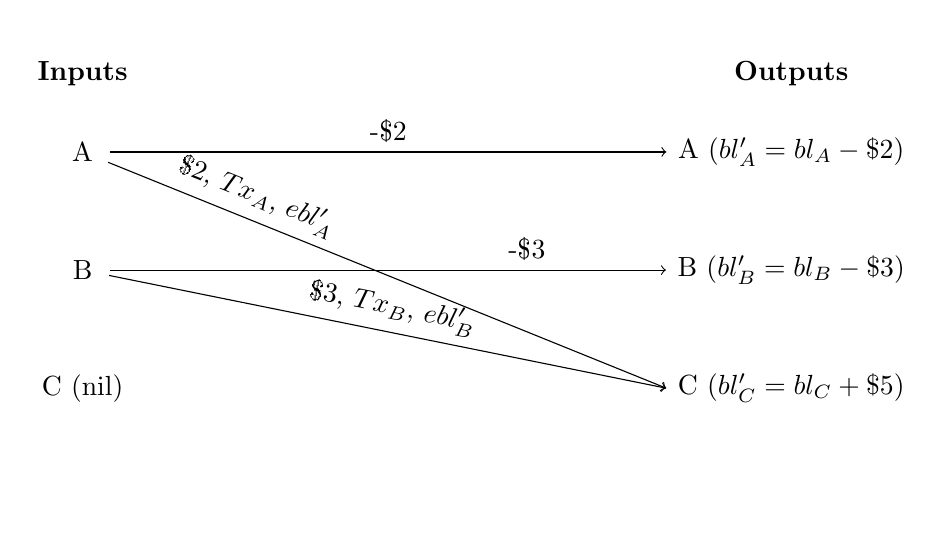
\begin{tikzpicture}
  \draw (0,1) node {\textbf{Inputs}};
  \draw (9,1)  node {\textbf{Outputs}};
  
  \node[shape=circle] (A) at (0, 0) {A};
  \node[shape=circle] (B) at (0, -1.5) {B};
  \node[shape=circle] (C) at (0, -3) {C (nil)};
  \node[shape=circle] (A') at (9, 0) {A ($bl_A' = bl_A - \$2$)};
  \node[shape=circle] (B') at (9, -1.5) {B ($bl_B' = bl_B - \$3$)};
  \node[shape=circle] (C') at (9, -3) {C ($bl_C' = bl_C + \$5$)};
  \draw[->] (A) -- (A') node [midway, above, sloped] {-\$2};
  \draw[->] (A) -- (C'.west) node [near start, above, sloped] {\$2, $Tx_A$, $ebl_A'$};
  \draw[->] (B) -- (B') node [near end, above, sloped] {-\$3};
  \draw[->] (B) -- (C'.west) node [midway, above, sloped] {\$3, $Tx_B$, $ebl_B'$};
\end{tikzpicture}
\end{center}
\label{payment_example}
\caption{Payment Example}
\end{figure}

The payment protocol between two parties is done as the Figure \ref{payment}.

\begin{figure}[h]
\begin{center}
  \begin{tikzpicture}
    \matrix (m) [matrix of math nodes, nodes in empty cells,
                 row sep=0.5cm,
                 column sep=4cm,
                 minimum width=4cm] {
      \textbf{Payer (A)} & \textbf{Payee (B)} \\
      \begin{minipage} {5cm}
        $bl_A' = bl_A - \textsf{amount}$ \\
        $ebl_A' = u^{\beta_A'} g^{bl_A'}$
      \end{minipage}  & \\
                      & \\
                      & \begin{minipage} {4cm}
                          VerifyTx($\textsf{Tx}_A$) \\
                          $bl_B' = bl_B + \textsf{amount}$ \\
                          $ebl_B' = u^{\beta_B'} g^{bl_B'}$ \\
                          $\textsf{PoB}_B \leftarrow \text{ perform } PoB$ \\
                        \end{minipage} \\
                     & \\
      \begin{minipage}{5cm}
        construct $\textsf{Tx}_A'$ \\
        $\textsf{wo}(Q, \langle ebl_A, H(\textsf{Tx}_A') \rangle, \textsf{Tx}_A)$ \\
      \end{minipage} & \\
                     & \\
                     & \begin{minipage} {4cm}
                         VerifyTx($\textsf{Tx}_A'$) \\
                       \end{minipage} \\
    };

    \draw [-, transform canvas={yshift=0.5cm}] (m-1-1.west) -- (m-1-2.east);
    \draw [->] (m-3-1) -- (m-3-2) node [midway, above] {$\textsf{amount}, \textsf{Tx}_A$};
    \draw [<-] (m-5-1) -- (m-5-2) node [midway, above] {$ebl_B, ebl_B', \textsf{PoB}_B$};
    \draw [->] (m-7-1) -- (m-7-2) node [midway, above] {$\textsf{Tx}_A'$};
  \end{tikzpicture}
\caption{Payment Protocol}
\label{payment}
\end{center}
\end{figure}

$\textsf{Tx}_A$ is a transaction that has created $bl_A$. The payer subtracts the amount from the current balance ($bl_A$) and creates a new (encrypted) balance ($ebl_A'$). The payee adds the amount to the current balance ($bl_B$) and perform $PoB$ on the new balance ($bl_B'$). The payer constructs a new transaction combining the encrypted balances and PoBs of both parties, then writes it to the quorum. (See the following section for {\sf wo}.) \textsf{Tx} is verified during the protocol as the Algorithm \ref{VerifyTx}.
\begin{algorithm}[h]
\label{VerifyTx}
\caption{VerifyTx}
\KwIn{$Tx$: Transaction of $ebl$}
\KwOut{true/false}
\SetKw{Continue}{continue}
\SetKwFunction{VerifyTx}{VerifyTx}
\SetKwProg{Fn}{Function}{:}{}
\Fn{\VerifyTx{Tx}} {
  \ForEach{$i \in $Tx} {
    \If {PoB.Verify(Tx.$PoB_i$) = failed} {
      \Return{false}
    }
    \If {$\textsf{read}(Q, \textit{Tx}.ebl_i) \ne H(\textit{Tx})$} {
      \Return{false}
    }
  }
  \Return {$(\prod_i PoB_i.e) / (\prod_i PoB_i.e') \overset{?}{=} \prod_i PoB_i.w$}
}
\end{algorithm}

\subsection{Write Once with PoB}
In {\sf bftkv}, to write a variable to a quorum the client signs the tuple with its own Quorum Certificate so it enforces the TOFU policy. In other words, the client becomes the owner of the variable. But with the Write Once property the variable will never be modified in any way therefore such ownership does not make much sense. We extend the write function for \textsf{Tx}. Instead of signing the tuple with QC we use PoB to guarantee the validity of the key ($ebl$) - value (\textsf{Tx'}). The Quorum Clique runs the Algorithm \ref{VerifyTx} over \textsf{Tx} and if it verifies it signs the tuple:
\[
\textsf{wo}(QC, \langle ebl, \textsf{Tx}' \rangle, \textsf{Tx}) \longrightarrow \sigma_i = \textit{Sign}(\langle ebl, H(\textsf{Tx}') \rangle).
\]
The client collects the signatures ($S = \{\sigma_i\}_{i \in QC}$) from the QC and write it to the KV quorum:
\[
\textsf{write}(KVQ, \langle ebl, H(\textsf{Tx}') \parallel H(\textsf{Tx}) \rangle, S).
\]

The KV quorum checks equivocation the same manner as the usual case so double spending will be detected with the possibility analyzed in \textsf{bftkv} \cite{bftkv}. Not only that, the quorum system prevents replay attacks as well. The key $ebl$ is used only once for a specific \textsf{Tx}. If someone copies $(ebl, ebl', \textsf{PoB})$ and makes up a new \textsf{Tx'} it will be different than the original \textsf{Tx} that has consumed $ebl$, so the attack will be detected.

\subsection{Audit}
\label{Audit}
The key ($ebl$) / value ($Tx$) pairs form a DAG. The topological order is guaranteed -- a new balance must be created from existing balances, except the genesis. In the Figure \ref{dag}, when $ebl_4$ is spent, $Tx_2$ is verified as {\sf VerifyTx}($Tx_2$). It is not necessary to track back beyond $ebl_3$ or $ebl_1'$ as when they are spent (i.e., written to the quorum) the past transactions must have been verified in the same manner.

\begin{figure}[h]
\begin{center}
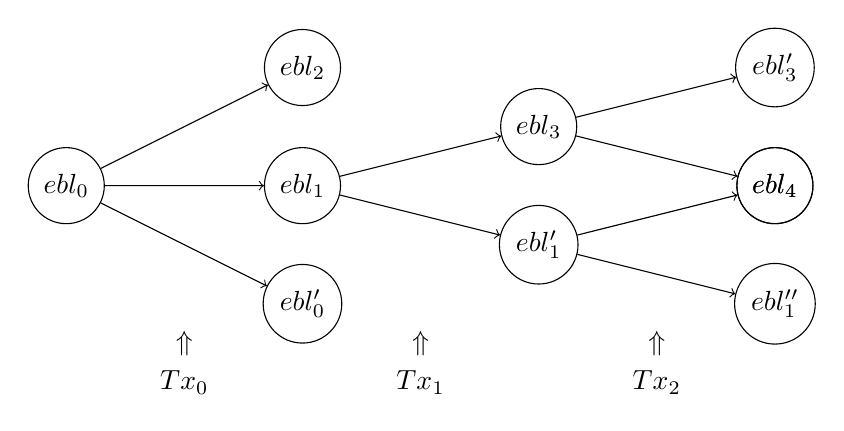
\begin{tikzpicture}[grow=right, every node/.style={draw,circle}, level distance=3cm, edge from parent/.style={->,draw}]
  \node (0) {$ebl_0$}
  child {node (0') [] {$ebl_0'$}}
  child {node [] {$ebl_1$}
    child {node (1') {$ebl_1'$}
      child {node {$ebl_1''$}}
      child {node {$ebl_4$}}}
    child {node {$ebl_3$}
      child {node {$ebl_4$}}
      child {node {$ebl_3'$}}}
  }
  child {node [] {$ebl_2$}};

  \begin{scope}[every node/.style={}]
    \path (0' -| 0) ++(+1.5cm, -1cm) node {$Tx_0$} ++(0,+0.5cm) node {$\Uparrow$};
    \path (0' -| 0') ++(+1.5cm, -1cm) node {$Tx_1$} ++(0,+0.5cm) node {$\Uparrow$};
    \path (0' -| 1') ++(+1.5cm, -1cm) node {$Tx_2$} ++(0,+0.5cm) node {$\Uparrow$};
  \end{scope}
\end{tikzpicture}
\caption{Balance Chain}
\label{dag}
\end{center}
\end{figure}

But, what if the quorum system is corrupted or the payer is somehow able to trick the quorum? In this case his balance might have been created out of thin air. As the security analysis of \textsf{bftkv}, even if faulty nodes outnumber the threshold it is still possible to detect the equivocation and in the transaction case, it will immediately invalidate the balance and abort the transaction. But, even if the probability is low there must be some fail-safe mechanism.

When an balance ($ebl$) is written to a quorum each member verifies \textsf{PoB} of the transaction that has created $ebl$, then store the hash value of the new transaction that spends $ebl$. Once \textsf{Tx} is verified it can be disposed. Since \textsf{Tx} is verified anyone who reads the variable ($ebl$) knows the value ($H(\textsf{Tx'})$) is valid without backtracking the balance to the genesis, but because of the above concern it would be good to have a way to validate it without relying on the quorum. We propose to have an archive service of \textsf{Tx} for this purpose. It is possible to keep \textsf{Tx} of all transactions in each quorum member but it can be too big and it is not necessary to keep the replication. The archive service is a simple key value store that takes $ebl$ and returns \textsf{Tx}. The client checks if $\textsf{ReadArchive}(ebl) = H(\textsf{Tx})$ and verifies each \textsf{PoB} in \textsf{Tx}.
The audit can be done as the Algorithm \nameref{AuditAlgo}.

\begin{algorithm}[h]
\label{AuditAlgo}
\caption{Audit}
\KwIn{$Tx$: Transaction of $ebl$}
\KwOut{true/false}
\SetKw{Continue}{continue}
\SetKwFunction{VerifyTxDeeply}{VerifyTxDeeply}
\SetKwProg{Fn}{Function}{:}{}
\Fn{\VerifyTxDeeply{Tx}} {
  \ForEach{$i \in $Tx} {
    \If {Tx.$ebl_i$ is genesis} {
      \Continue
    }
    \If {PoB.Verify(Tx.$PoB_i$) = failed} {
      \Return{false}
    }
    \If {$\textsf{read}(Q, \textit{Tx}.ebl_i') \ne H(\textit{Tx}) \vee \VerifyTxDeeply(\textsf{ReadArchive}(\textit{Tx}.ebl_i)) = \text{false}$} {
      \Return{false}
    }
  }
  \Return {$(\prod_i PoB_i.e) / (\prod_i PoB_i.e') \overset{?}{=} \prod_i PoB_i.w$}
}
\end{algorithm}

\subsection{Anonymity}
\textsf{Tx} does not include any information that can be linkable to users or devices. The balance is encrypted so it cannot be a clue to track transactions. However, the payment protocol is peer to peer, which means the payers and payees know each other's identity. $ebl$ can be linked to such identity even if it is pseudonym and we cannot anonymize them who are involed in the payment. The question is $ebl$ can be traceable? Basically \textsf{Tx} has $n$ pairs of input / output. When you get \textsf{Tx} from the archive service, you know $ebl$ is one of the \textsf{outputs} but you do not know what input is corresponding to it. (Also it can be newly created with that transaction, where the input is \textsf{nil}.) The same can be said for the forward direction. By getting \textsf{Tx} of $ebl'$ you can trace it forwardly but you do not know what output is corresponding to the input. In theory if someone wants to trace a balance he will need to keep tracking $\prod_i^{\textsf{gen}} \textsf{Tx}_i.n$ balances for \textsf{gen} generations, which is $\Omega(2^{\textsf{gen}})$.

If the transaction chain is short and simple it can be possible to guess the path of a specific transaction. A simple mitgation is to add ``dummy'' balances that have 0 value to both inputs and outputs just to obscure the actual transaction. Such dummy balances can be consumsed in other transactions without affecting other balances to make the trace difficult. This makes Audit more inefficient as well though.

\section{Wallet}
The payment scheme does not require any long term keys such as signing keys. Instead, each balance has a corresponding witness $(\beta_{\triangle}, bl, \gamma)$. The balance ($bl, \gamma$) can be outside of HW and the range proof can be calculated in AP. Only $\beta_{\triangle}$ has to be stored in the HW. In the ZK protocol only $(t_5, v_{5i}, z_{5i})$ is calculated inside the HW.

Wallet can participate in the KV quorum. Each memeber keeps the hash value of only leaves in the Balance Chain. The intermediate nodes are needed for audit but nodes like Wallet do not have to keep them. This could make the payment faster as the payee can verify the payer's balance offline if it hits the local KV store. Eventually the payee has to check if the payer has written the transaction to the quorum but it could give a flexibility to the settlement. More importantly, if Wallet participate the KV quorum will be much bigger, and it will make the entire system more robust. See the security anaylysis of \textsf{bftkv}. Also Wallet is the most trustworthy entity, because it is only for you and you trust it, so you do not have to worry about faulty KV nodes trying to trick you.

\section{Bootstrap from Bitcoin}
This is a payment scheme, not a cryptocurrency. There is no mining that makes money. It needs other digital currency systems to make the genesis balance. Using Bitcoin as the currency model, the genesis balance can be created as follows:

\begin{figure}[H]
\begin{center}
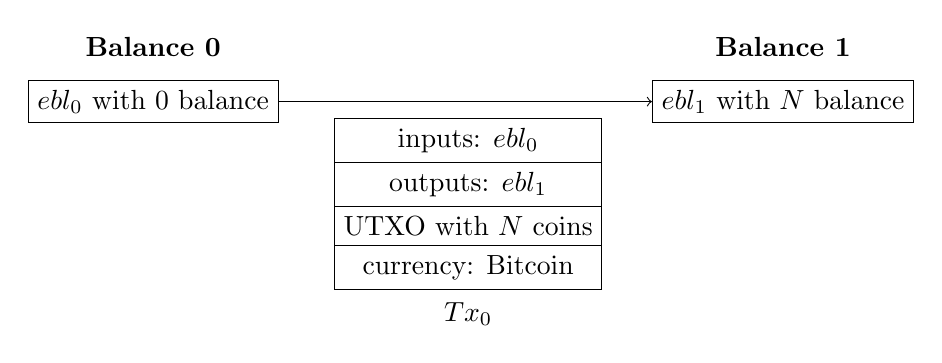
\begin{tikzpicture}[stack/.style={rectangle split, rectangle split parts=#1, draw, anchor=center}]

  \draw (0, 0.7) node {\textbf{Balance 0}};
  \node[draw] (A) at (0,0) {$ebl_0$ with 0 balance};

  \node[stack=4,
        every one node part/.style={fill=gray}] (B) at (4, -1.3) {
    \nodepart{one} {inputs: $ebl_0$}
    \nodepart{two} {outputs: $ebl_1$}
    \nodepart{three} {UTXO with $N$ coins}
    \nodepart{four} {currency: Bitcoin}
  };
  \draw (4, -2.7) node {$Tx_0$};

  \draw (8,0.7) node {\textbf{Balance 1}};
  \node[draw] (C) at (8,0) {$ebl_1$ with $N$ balance};

  \draw[->] (A) -- (C);

\end{tikzpicture}
\end{center}
\label{bootstrap}
\caption{Bootstrap from Bitcoin and Fiat Currency}
\end{figure}

The UTXO sends $N$ coins to the public address owned by the quorum. To convert the balance back to bitcoin, the user makes a transaction for $0$ balance so the system will make a UTXO to send the amount of the last balance to the user's address.
This payment scheme is all about the balance. The amount of all bitcoins deposited to the public address must be exactly the same as the total balance of all the balance chain, therefore withdrawing has to be done without any shortage.
Also, we use the distributed signing feature of {\sf bftkv} to manage the private key of the public address. The signing key is distributed to the quorum using the threshold cryptography technique and never be revealed during the signing process. See ``3.4 Distributed Signing'' \cite{bftkv}.

\subsection{Stablecoins}
As in the Figure \ref{bootstrap}, the ``currency'' field is introduced to indicate what currency is the origin of the balance. All transactions derived from the genesis balance has to inherit the currency. It is inhibited to make a transaction between balances that have different currency. This way the total assets of the same currency in the blockchain is assured to cash out. Exchanges between currencies is out of scope.

The currency is encoded in the balance $bl$ such as $\textsf{currency} \times 2^d + bl$, where \textsf{currency} is encoded to a small integer like $1..127$. This way it is easy to verify all balances have been created with the same currecy, by dividing $ebl$ by $g^{\textsf{currency} \times 2^d}$.

% \section{Smart Contracts and API}
% Our system is based on Byzantine fault tolerant protocols. Unless the integrity of the program (smart contracts) is guaranteed it is difficult to guarantee the BFT property. It is easy to verify the integrity {\em statically} using the blockchain technologies but this does not guarantee that the program is really executed as-is. In this regard, The blackbox property \cite{blackbox} or indistinguishability obfuscation is too strong for the code integrity 

\begin{thebibliography}{99}

\bibitem{bftkv}
  Ryuji Ishiguro, ``A Byzantine Fault-tolerant KV Store for Decentralized PKI and Blockchain'' \url{https://github.com/yahoo/bftkv/blob/master/docs/bftkv.pdf}

\bibitem{pbft}
  Miguel Castro and Barbara Liskov, ``Practical Byzantine Fault Tolerance''

\bibitem{byzantinequorum}
  Malhi, D. and Reiter, M. (1998) ``Byzantine Quorum Systems''

% \bibitem{blackbox}
% Barak, B., Goldreich, O., Impagliazzo, R., Rudich, S., Sahai, A., Vadhan, S., and Yang, K. (2001) On the (Im)possibility of Obfuscating Programs.

\end{thebibliography}

\end{document}
